\documentclass[main.tex]{subfiles}
\begin{document}

\chapter{NEMO detectors}


\NI Initiated in the late 1980s, the main aim of the NEMO project is the search for 0$\nu\beta\beta$. The strategy adopted by the collaboration is the direct detection of the 2 electrons emitted in $\beta\beta$ decay. A strategic point in the search for these very rare processes is the background level. The detectors must be installed in underground laboratory to be protected from the cosmic rays but also all the materials enter in the detector fabrication have to be radiopure.


\bigskip


\NI This chapter presents the different phases and the different prototypes built by the NEMO collaboration. The principe of the NEMO detection is presented in Section~\ref{sec:Principe}. Section~\ref{sec:LSM} shortly describes the Modane undergound laboratory where the NEMO detectors were hosted. The 2 first prototypes NEMO-1 and NEMO-2 are presented in Section~\ref{sec:NEMO1-2}. Section~\ref{sec:NEMO3} and \ref{sec:SuperNEMO} describe respectively the NEMO-3 detector and the SuperNEMO project.


\section{Historical and principle}





\subsection{Principe}\label{sec:Principe}


To directly detect the 2 electrons emitted in $\beta\beta$ decay, the $\beta\beta$ sources consist of thin foils placed at the center of the detector and surrounded by a tracking device for electron track reconstruction. The tracking volume is itself surrounded by a calorimeter for electron energy measurement. Figure~\ref{SchemaNEMOl} presents the detection principle of $\beta\beta$ event combining tracking and calorimetric measurement. This unique feature allow a full reconstruction of the different parameters of the events. The energy of each particle can be measured independently also as the angles between the particle tracks, which allows the discrimation between the processes behind $\beta\beta$ decay and a good background discrimination. Futhermore, this approach permits to search for the 0$\nu\beta\beta$ decays among several isotopes. 


\begin{figure}[h!]
\begin{center}
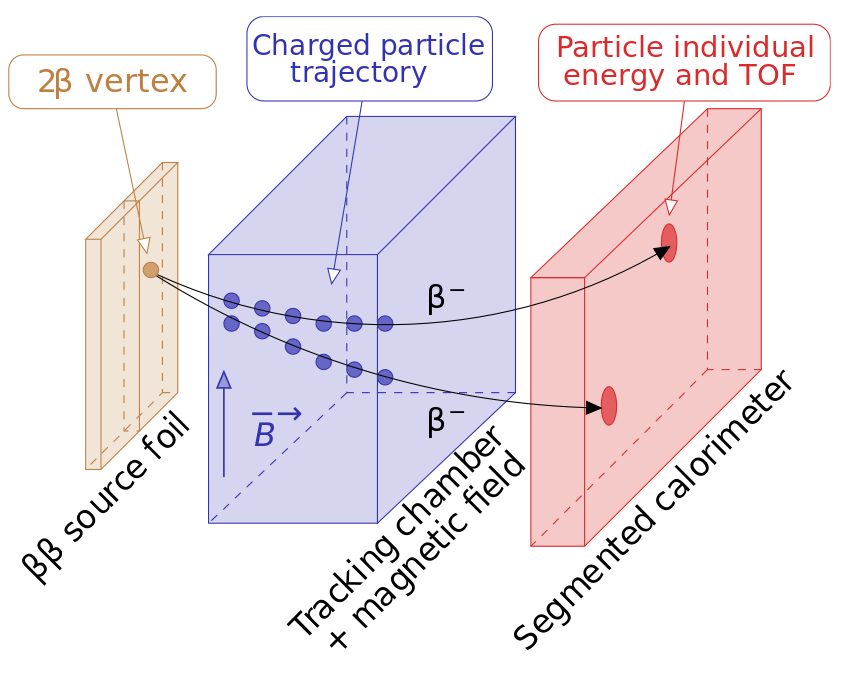
\includegraphics[scale=0.30]{pictures/Chap3/SchemaNEMO.png}
\caption{Detection principe of a $\beta\beta$ event combining tracking and calorimetric measurement. A thin $\beta\beta$ source is placed at the center of the detector. A tracking chamber allied with a magnetic field reconstruct the particle trajectory. The particle energy and their time of fligh is obtained with a calorimeter.}
\label{SchemaNEMOl}
\end{center}
\end{figure}


\subsubsection{$\beta\beta$ source foils}


\NI The $\beta\beta$ source foils of the NEMO project are the central part of the detectors. They can be metallic or composite but in anycase a great care is taken in their fabrication, and more particularly about their radio-purity. The foils must be the thinest as possible to avoid energy loss of the leaving particles. On the other hand, they have to be strong enough to withstand all the time of the experiment. More details about the source foils and their fabrication will be given in the next sections.


\subsubsection{Tracking volume}


\NI The tracking device of the NEMO experiments is a wire chamber working in Geiger mode coupled with a magnetic field for charge discrimination. Each Geiger cell is composed by a central wire (called anode) and surrunded by 8 wires distributed on an circle (cathode), a voltage difference is applied between the cathode and the anode.


\bigskip


\NI When a charged particle crosses the tracking volume, the gas is ionized by photoelectric effect. Due to the high voltage, the created electrons will migrate to the anode and be multiplied in a avalanche. Some photons are also emitted and generate other avalanches, this chain reaction is called Townsend avalanche, shown in Figure~\ref{avalancheTownsend}. For a short time, the gas is conductive, and the plasma propagates along both side of the anodic wire. The arrival time of the plasma at the endcaps provides informations on the longitudinal distance of the particle interaction point. The radial position to the anode is determine by the drift time (in this case a trigger is necessary which is given by the calorimeter). By knowing the longitudinal and radial distance of several Geiger cells, the particle 3-D track can be reconstructed. The discharge ends when the positive ions concentration is high enough to counterbalance the electric field. A schematic view of a Geiger cell and the expected anodic and cathodic signals are shown in Figure~\ref{trackerSignal}. 


\begin{figure}[h!]
\begin{center}
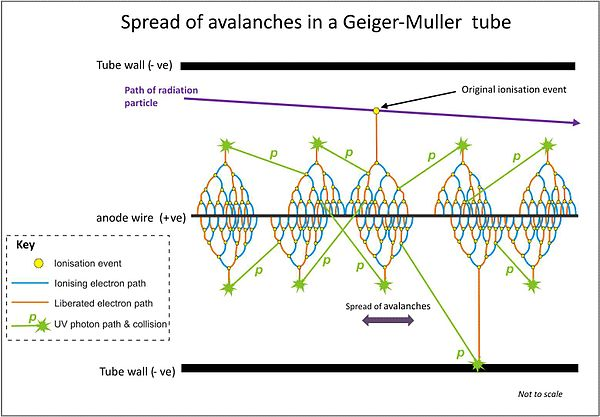
\includegraphics[scale=0.70]{pictures/Chap3/avalanche.jpg}
\caption{Picture explaining a Townsend avalanche, an incident particle interacts in the gas and ionize it. The created electron drifts to the cathodic wire due to the electric field and generates an avalanche. Some emitted photons can also ionize the gas and create another avalanche.}
\label{avalancheTownsend}
\end{center}
\end{figure}


\NI In most of the case, the wire chambers are filled with a noble gas because of their interesting characteristics. They are mono-atomic (no rotation or vibration), easy to purify and not electronegative. At the end of the discharge, during the recombinaison, an electron can be extracted from the cathode and re-create an avalanche. To avoid this phenomena, a small amount of a quenching gas is added.


\bigskip


\NI The great gain of the Geiger mode (between 10$^\text{6}$ and 10$^\text{8}$) allows to reach high sensitivity detection but unfortunately does not allowed to know the nature of the particle and their energy. Another drawback of the wire chambers working in Geiger mode is the long dead time (few hundred $\mu$s). This dead time is not an obstacle in NEMO detector since the rate is expected to be at the Hertz order.    




\begin{figure}[h!]
\begin{center}
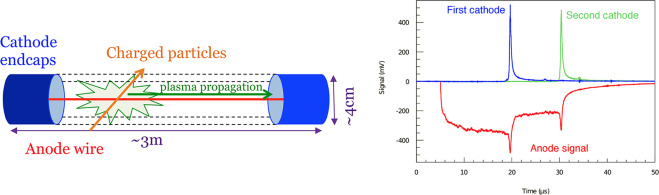
\includegraphics[scale=0.80]{pictures/Chap3/trackerSchema.jpg}
\caption{Left : Geiger cell of the tracker. The red line represents the anode wire surrended by 8 cathode wires attached to cathod endcaps (represented by the dashed lines). Right : anodic and cathodic signals detected.}
\label{trackerSignal}
\end{center}
\end{figure}



\subsubsection{Calorimeter}


\NI The calorimeter of NEMO experiments is composed of plastic scintillator blocks coupled with photomultiplier tubes (PMT). By interacting inside the block, a particle will excite the electrons of the medium which will de-excite by emitting visible light. This scintillation light is then collected by a PMT. The energy of the incident particle can be determine thanks to the amount of scintillation light. In case of plastic scintillator only a small fraction of the kinetical energy of the incident particle is converted in light. The majority of the energy leaves under a non radiative way (phonon, heat). The light yield per path length (dL/dx) can be estimated with the Birks' law : 


\begin{equation}
\frac{\text{dL}}{\text{dx}} = \frac{\text{S}~(\frac{\text{dE}}{\text{dx}})}{\text{1}+\text{k}_\text{B}~(\frac{\text{dE}}{\text{dx}})}
\end{equation}


\NI where S is the scintillation efficiency, dE/dx is the energy loss of the particle per path length and k$_\text{B}$ is the Birks' constant which depends on the scintillator material. 


\bigskip


\NI A part of the scintillation light can be re-absorbed by the block material. In order to avoid this phenomena another materials can be introduced inside the block to shift the wave length. This wave length shifter composent improve the transparency and also has the advantage of emitting light in the acceptance range of the PMT. 


\bigskip


\NI Coupled directly or indirectly (a light guide can be interposed) to the scintillation block, a PMT recovers the light to convert it into an electric signal. A PMT is made of a photocathode, dynodes and an anode placed in a vacuum tube. The photocathode converts the incident photons by photoelectric effect into low energetic electrons in a linear yield. At this stage, the number of photo-electrons is still too low to provide an electric signal. These photo-electrons are directed to the first dynode thanks to the focusing electrode where they will be multiplied. By putting dynodes one after the other and appliying an higher positive voltage than the previous one, the signal is highly amplify. The collected signal by the anode is proportionnal to the energy of the incident photon. Figure~\ref{PMT} presents a simplified view of a PMT.


\begin{figure}[h!]
\begin{center}
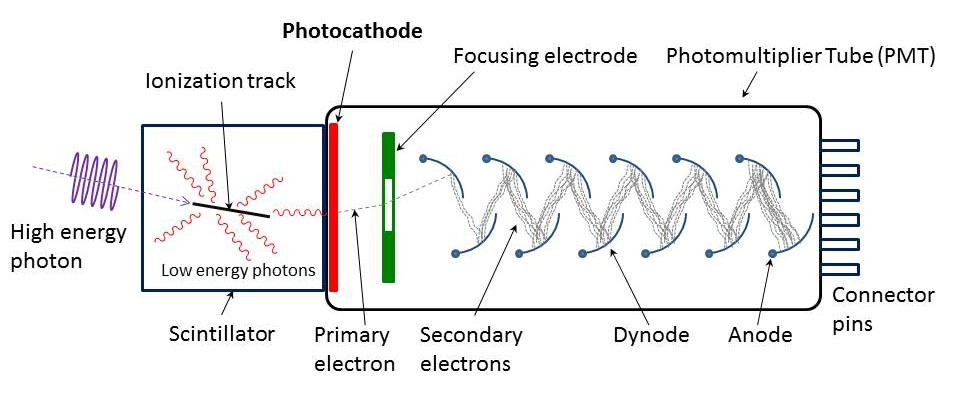
\includegraphics[scale=0.35]{pictures/Chap3/PhotoMultiplierTubeAndScintillator_v2.jpg}
\caption{Simplified view summarizing the operation of a photomultiplier.}
\label{PMT}
\end{center}
\end{figure}


\bigskip


\NI In general a PMT is sensitive in ultraviolet and near infrared and have a very short response time (tens of ns). A PMT can be characterized by its quantum efficiency, its collection efficiency and its multiplication factor. The quantum efficiency ($\epsilon_\text{q}$) is the probability for an incindent photon to produce a photo-electron. Today, $\epsilon_\text{q}$ rarely  exceeds 20-30 \% and depends of the photon wavelength. In the electron multiplication mechanism, some electrons may deviate from their favorable trajectories and not contribute to the multiplication. This effect can be parametrized by the collection efficiency ($\epsilon_\text{c}$) which depends on the geometry and composition of the dynodes. Finally, the multiplication factor ($\delta$) is defined for each dynode as the ratio of number of emitted electrons by the number of incindent electrons.


\bigskip


\NI In the case where PMT is used in a strong magnetic field, the electron trajectories are curved and steer them away from the dynoded. That is why the PMT are often shielded with soft iron or $\mu$-metal. 


\FloatBarrier


\subsection{Modane underground laboratory}\label{sec:LSM}


\NI The Modane underground laboratory (LSM : Laboratoire Souterrain de Modane in french) is located in the Frejus tunnel at the border between France and Italy (Figure~\ref{LSMtunnel}).  Sheltered from cosmic rays, the laboratory have been inaugurated in 1982 under 1700~meters of rocks (4200 meter water equivalent) which makes it the deepest underground laboratory in Europe and the third one in the world. The cosmic ray flux inside the laboratory have been estimated to be 4.m$^\text{-2}$.j$^{\text{-1}}$, compared to the million of particles arriving per m$^\text{2}$ at the surface of the Earth. Figure~\ref{LabDeepth} shows the total muon flux according the depth for different underground laboratory around the world. 


\bigskip


\begin{figure}[h!]
\begin{center}
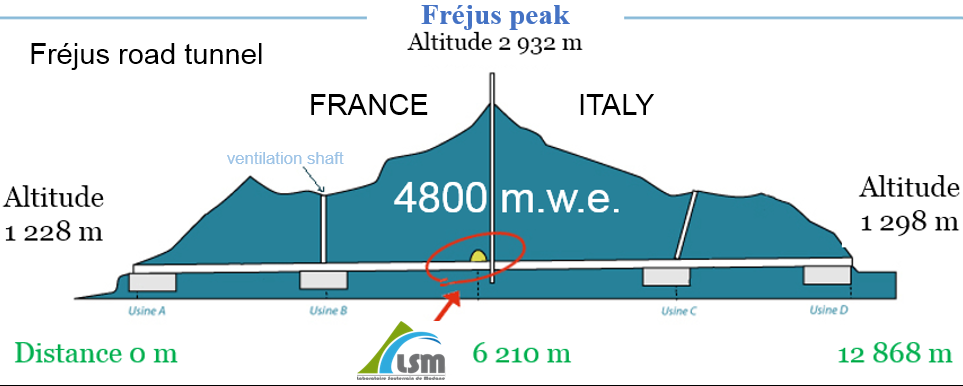
\includegraphics[scale=0.40]{pictures/Chap3/LSMtunnel.png}
\caption{Schematic view of the Modane underground laboratory location in the Frejus tunnel.}
\label{LSMtunnel}
\end{center}
\end{figure}


\NI The protected environment of the laboratory is very conducive to the searches requiring a very low background. Initially, the laboratory hosted an experiment searching for the proton decay. Latest, the laboratory diversified its activities, including astrophysics (mainly for the searches for the dark matter), biology, geology, electronics and environmental studies. The laboratory also have several High Purity Germanium detectors (HPGe) to measure very low radioactivity. 


\begin{figure}[h!]
\begin{center}
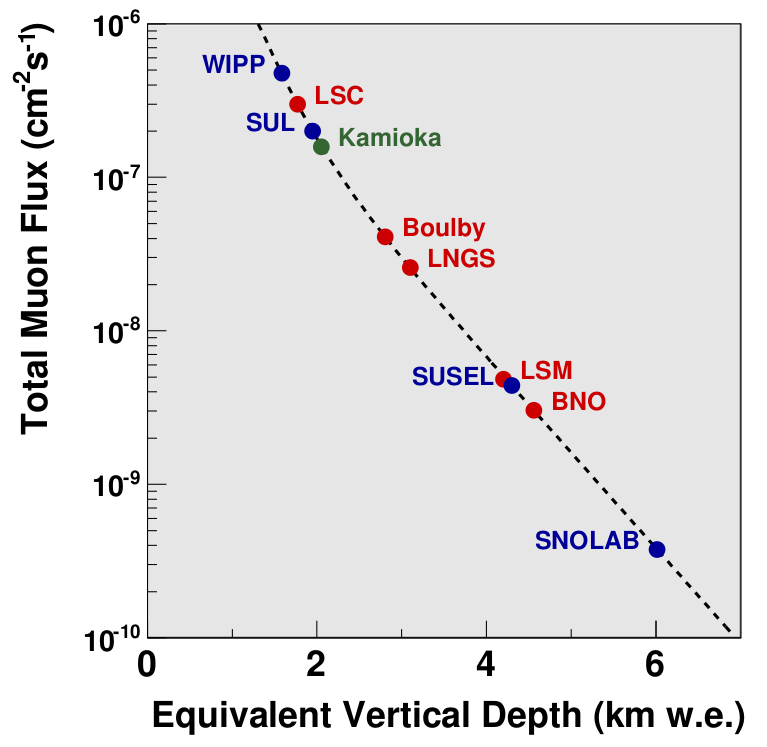
\includegraphics[scale=0.27]{pictures/Chap3/lab_depth.png}
\caption{Total muon flux in cm$^{\text{-2}}$.s$^{\text{-1}}$ with respect to the depth for different underground laboratory.}
\label{LabDeepth}
\end{center}
\end{figure}


\NI LSM hosted NEMO-2 detector at the end of the 80's. Then NEMO-3 have been installed and took data between 2003 and 2011. Today NEMO-3 have been replaced by SuperNEMO demonstrator which is currently under construction and commissionning phase.


\FloatBarrier


\subsection{NEMO-1 and NEMO-2}\label{sec:NEMO1-2}


\NI Before to build a large scale detector, the collaboration wanted to ensure validity of electron reconstruction at low energy with the tracking device. Two prototypes have been built, NEMO-1 and NEMO-2, which also allow to understand important points for improving the sensitivity of the future detectors. 

\subsubsection{NEMO-1}

\NI The first prototype NEMO-1 was built in 1988. In a first step, the detector took data with cosmic at the sea level and then  have been moved at LSM where it worked during 18 months. NEMO-1 demonstrated that the track reconstruction of the low energetic electrons is possible until few hundred keV. This prototype was also useful to study the shielding and to measure the radioactivity inside the wire chamber.


\bigskip


\NI The trajectory of the electron was reconstructed thanks to 64 Geiger cells made of a central wire surrounded by 8 ground wires of 1 meter long (8 $\times$ 8). The tracker volume was filled with gaseous helium and 2\% of ethanol as quencher. The final gas density was 0.2 mg.cm$^{\text{-2}}$ which limit the energy loss of the electron (loss of 14 keV for an electron of 1 MeV crossing 50~cm of the gas).


\bigskip


\NI The energy of the electrons was measured thanks to 2 plastic scintillators planes surrounding the tracker volume and measuring 0.28 $\times$ 0.02 $\times$ 1.0 m$^{\text{3}}$. Each plane was divided into 2 parts coupled with a PMT. 


\bigskip


\NI To be protected from the background, the detector was shielded with iron and lead for a total width of 20~cm lead equivalent.


\subsubsection{NEMO-2}


NEMO-2 is the second prototype built by the collaboration. Around 10 times bigger than NEMO-1, its main goal was the study of the background and the validation of the strategy to measure them via different channels. A schematic view of the detector is presented in Figure~\ref{NEMO2}.


\begin{figure}[h!]
\begin{center}
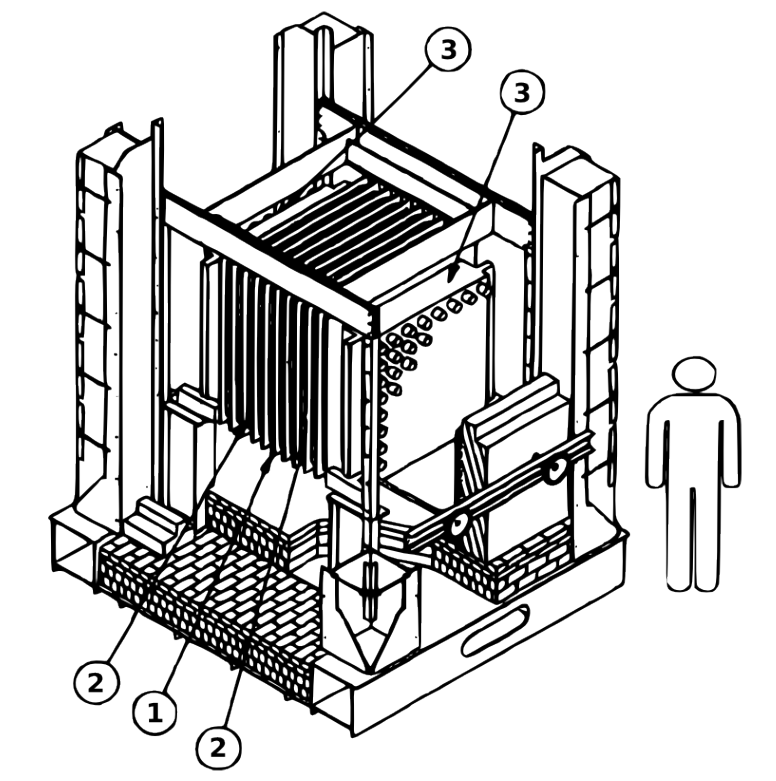
\includegraphics[scale=0.27]{pictures/Chap3/NEMO2.png}
\caption{Schematic view of the NEMO-2 detector. (1) central frame supporting the $\beta\beta$ source, (2) copper frame holding the Geiger cells, (3) 8 $\times$ 8 scintillators coupled to PMT.}
\label{NEMO2}
\end{center}
\end{figure}

\bigskip


\NI The source frame is the central part of the detector, labelled (1) in~Figure~\ref{NEMO2}. Measuring~1~m$^\text{2}$, this frame hold different $\beta\beta$ isotopes during several phases between 1991 and 1995. The results obtained for the double beta decay of these isotopes are summarized in Table~\ref{NEMO-2-results}.


\begin{table}[h!]
\centering
\begin{tabular}{c|c|c}
Isotope           & Mass (nat. + enr.) [g] &T$_{\text{1/2}}$ $\times$ 10$^{\text{19}}$ [y] at 90 \% C.L. \\[0.05cm]
\toprule
$^{\text{116}}$Cd & 143 + 152   & 3.75 $\pm$ 0.35 (stat.) $\pm$ 0.21 (syst.)  \cite{NEMO2:Cd116}\\[0.05cm]
$^{\text{100}}$Mo & 163 + 172   & 0.95 $\pm$ 0.04 (stat.) $\pm$ 0.09 (syst.)  \cite{NEMO2:Mo100}\\[0.05cm]
$^{\text{82}}$Se  & 134 + 157   & 8.30 $\pm$ 1.00 (stat.) $\pm$ 0.70 (syst.)  \cite{NEMO2:Se82}\\[0.05cm]
$^{\text{96}}$Zr  & 18.3 + 20.5 & 2.1 $^{+\text{0.8}}_{-\text{0.4}}$ (stat.) $\pm$ 0.2 (syst.) \cite{NEMO2:Zr96} \\[0.05cm]
\bottomrule
\end{tabular}
\caption{Results of the search for double decay with the NEMO-2 detector. The second column presents the isotope mass introduced (natural and enriched).}
\label{NEMO-2-results}
\end{table}  


\bigskip


\NI The source frame was surrounded on each side by 5 copper frames holding 640 Geiger cells (320 horizontal and 320 vertical), labelled (2) in~Figure~\ref{NEMO2}. The tracking volume was filled with gaseous helium and 4\% of ethanol for quenching. The transverse resolution was 500 $\mu$m and the longitudinal resolution was 4.7 mm. 


\bigskip


\NI The energy and the time of light of the electrons was obtained thanks to 2 planes of 8 $\times$ 8 plastic scintillators (for a total of 128 PMTs), labelled (3) in~Figure~\ref{NEMO2}. The distance between the source and the calorimeter was 50 cm. The dimensions of each scintillator block was 12~$\times$~12~cm$^{\text{2}}$ with a depth of 2~cm$^{\text{2}}$ to fully contain the electrons with an energy up to 4 MeV. Light guide was installed between scintillator and PMT. The calorimeter energy resolution (FWHM) was 18\% at 1 MeV with a time resolution of 275 ps (550 ps at 0.2 MeV). A laser and optical fiber was introduced close to PMTs to check the stability of the scintillation detectors. Finally, the tracking volume and scintillators were surrounded by a lead (5~cm) and iron (20~cm) shield.



\bigskip


\NI NEMO-2 demonstrated that the background coming from the radon was important and its reduction was crucial to scale the experiement up.   


\FloatBarrier


\section{NEMO-3}\label{sec:NEMO3}


\NI The NEMO-3 detector took data between January 2003 and January 2011 and search for $\beta\beta$ decays among 7 different isotopes.


\subsection{General design}

\NI NEMO-3 adopted a cylindrical geometry in order to optimise the volume of the detector with respect to the foils surface. The detector was divided into 20 identical sectors. A exploded view of the detector is shown in Figure~\ref{NEMO3Detector}.


\bigskip

\NI The sources were verticaly disposed forming a cylinder of 3.1 of diamater and 2.5 meters high for a total surface of around 20 m$^\text{2}$. Several isotopes in different proportion were placed in the detector. On each side of the source foil, a total of 6180 Geiger cells allow the track reconstruction in 3 dimensions. Plastic scintillators coupled with low radioactivity PMT surrounded the wire chamber. 


\bigskip


\NI A solenoid surrounding entirely the detector produced a 25~Gauss magnetic field parallel to the foil axis, in order to identify the particle charge. The detector was shielded from photons with 19~cm of iron, 30~cm of borated water on the sides parts and 28~cm of wood on the top and bottom sides thermalize fast neutrons and capture thermal neutrons.  


\begin{figure}[h!]
\begin{center}
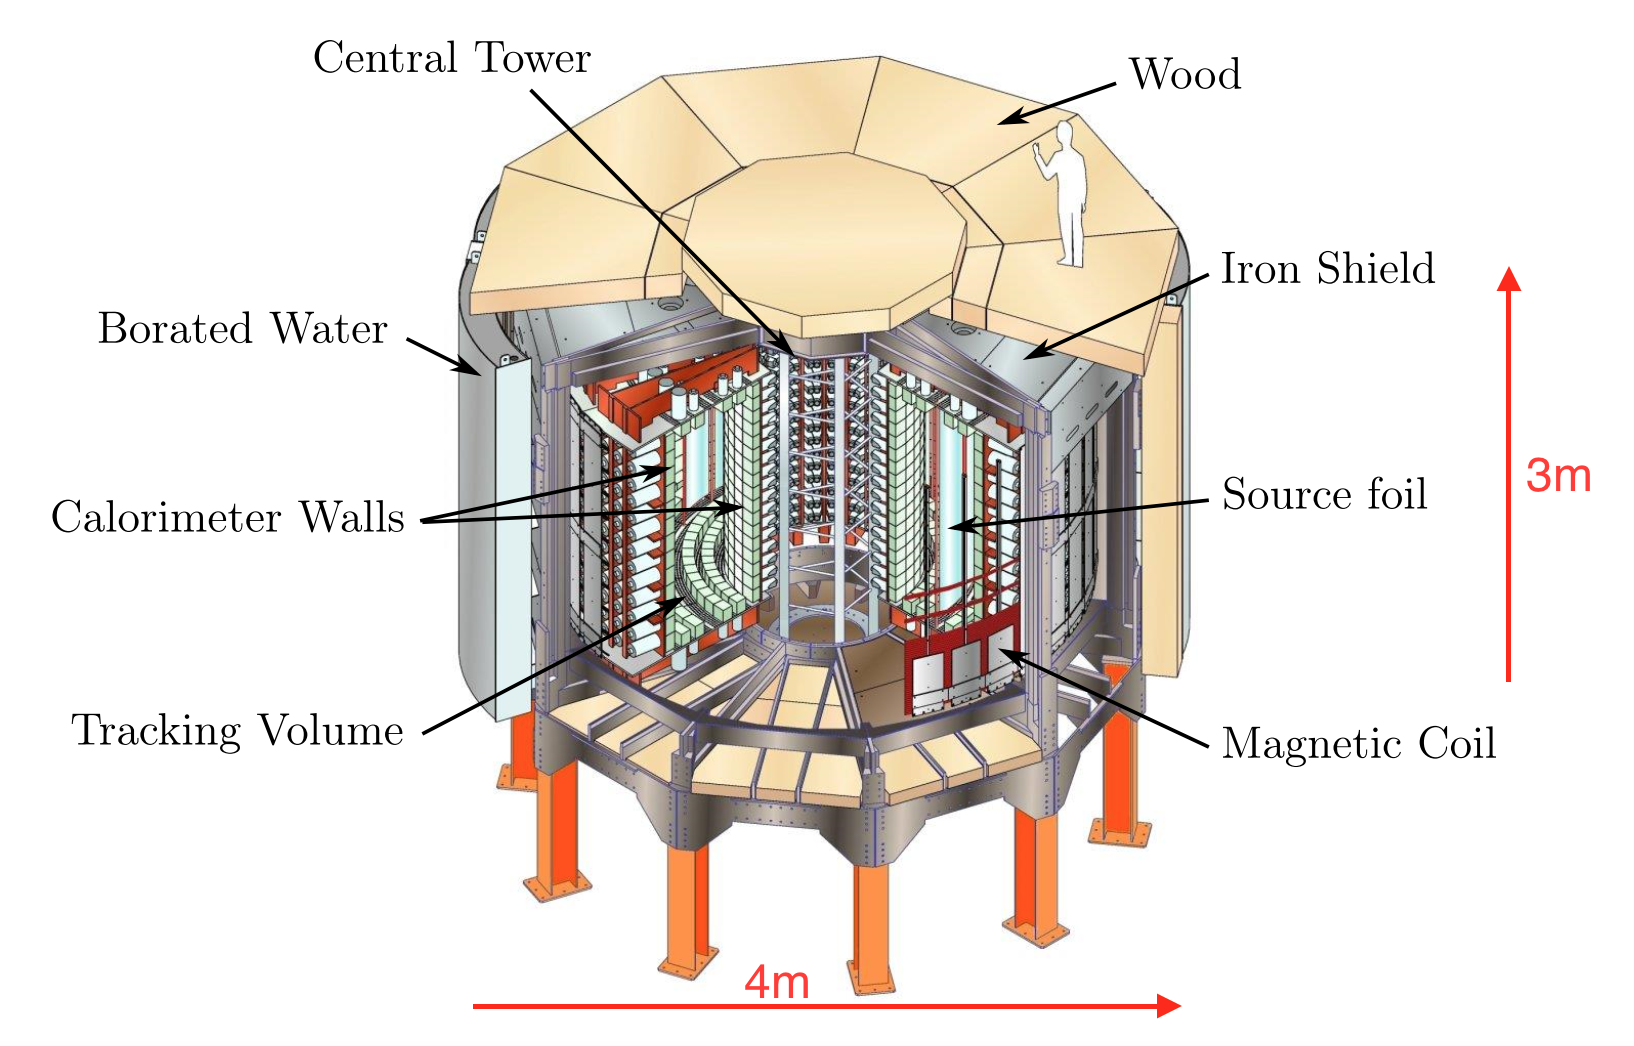
\includegraphics[scale=0.50]{pictures/Chap3/DetectorCrossSection.png}
\caption{Schematic view of the NEMO-3 detector.}
\label{NEMO3Detector}
\end{center}
\end{figure}


\begin{figure}[h!]
\begin{center}
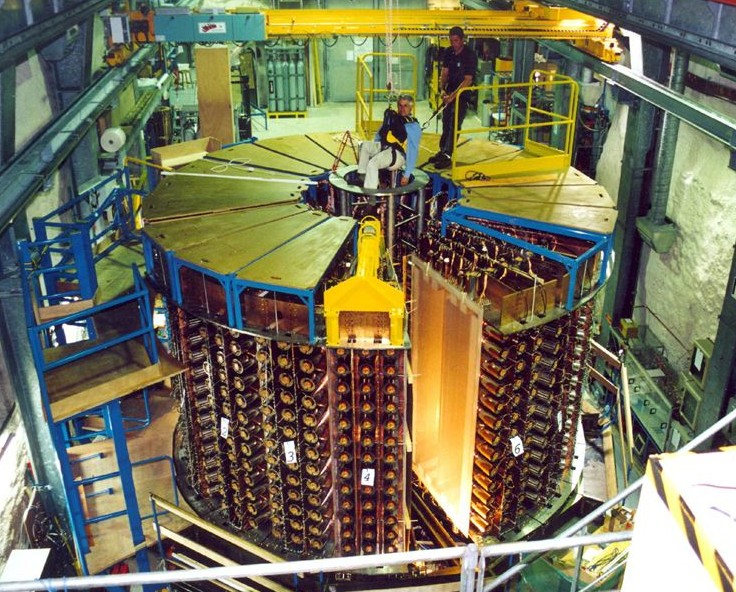
\includegraphics[scale=0.40]{pictures/Chap3/photoNEMO3.jpg}
\caption{Picture of the NEMO-3 detector in LSM before the installation of the last sector. The coil generating the magnetic field and the different shildings are not present.}
\label{NEMO3Photo}
\end{center}
\end{figure}


\FloatBarrier


\subsection{Source foils}

\NI The separation of the source foils from the rest of the detector give to NEMO-3 the great advantage to place different isotopes. This may allow to confirm a possible excess in the 0$\nu\beta\beta$ region with several atoms and test the results being less dependant of the nuclear matric element evaluations and by better controlling the backgrounds. The choice of which isotopes to study has mainly been determined by the following criteria (summarized in Table~\ref{tab:isotopeNEMO3} for the isotopes introduced in NEMO-3) : 


\begin{itemize}
\item the transition energy (Q$_{\beta\beta}$) : the higher this value is, the less the natural radioactivity is troublesome. The minimal value is 2.615~MeV which correspond to the higher $\gamma$-ray energy produced in natural radioactivity (decay of $^{\text{208}}$Tl).


\item the half-life of the 2$\nu\beta\beta$ process (T$_{\text{1/2}}^{\text{2}\nu}$) : the higher this value is, the less the number of 2$\nu\beta\beta$ events in the Q$_{\beta\beta}$ region is high.  


\item the natural isotopic abundance : in general the higher the abundance the easier the enrichment process. Only isotopic abundances greater than 2 \% were considered. 
\end{itemize}


\bigskip


\NI Five nuclei are quite satisfying : $^{\text{100}}$Mo, $^{\text{82}}$Se, $^{\text{116}}$Cd, $^{\text{96}}$Zr and $^{\text{150}}$Nd. The $^{\text{100}}$Mo (7~kg) and $^{\text{82}}$Se (0.9~kg) isotopes have been introduced for the search for 0$\nu\beta\beta$ decay. Smaller amount of $^{\text{116}}$Cd (405~g), $^{\text{150}}$Nd (37~g) and $^{\text{96}}$Zr (9.4~g) have also been inserted for 2$\nu\beta\beta$ decay studies. Even if $^{\text{48}}$Ca does not meet the criteria (very small natural abundance), $\sim$7~g have been introduced because of its impressive Q$_{\beta\beta}$ value which may allow a background free approach. 454~g of $^{\text{130}}$Te have also been added for 2$\nu\beta\beta$ studies (because of its high natural abundance). Foils made of copper (not a $\beta\beta$ emitter) and natural tellurium have been introduced in order to control the background measurements. The location of the sources among the different sectors are shown in Figure~\ref{NEMO3Sector}.


\bigskip



\begin{table}[h!]
\centering
\begin{tabular}{c|c|c|c|c}
Isotopes & Mass [g] & Q$_{\beta\beta}$ [MeV] & T$_{\text{1/2}}^{\text{2}\nu}$ [y] & Abundance [\%]\\[0.05cm]
\toprule
$^{\text{100}}$Mo & 6 914 & 3.034 & 7.2 $\times$ 10$^{\text{18}}$ & 9.63 \\[0.1cm]
$^{\text{82}}$Se  & 932   & 2.995 & 9.6 $\times$ 10$^{\text{19}}$ & 8.73 \\[0.1cm]
$^{\text{130}}$Te & 454   & 2.529 & 7.0 $\times$ 10$^{\text{20}}$ & 33.8 \\[0.1cm]
$^{\text{116}}$Cd & 405   & 2.802 & 2.9 $\times$ 10$^{\text{19}}$ & 7.49 \\[0.1cm]
$^{\text{150}}$Nd & 37    & 3.367 & 9.1 $\times$ 10$^{\text{18}}$ & 5.6  \\[0.1cm]
$^{\text{96}}$Zr  & 9.4   & 3.350 & 2.4 $\times$ 10$^{\text{19}}$ & 2.8  \\[0.1cm]
$^{\text{48}}$Ca  & 6.99  & 4.271 & 4.4 $\times$ 10$^{\text{19}}$ & 0.19 \\[0.1cm]
\bottomrule
\end{tabular}
\caption{Mass, Q$_{\beta\beta}$, T$_{\text{1/2}}^{\text{2}\nu}$ and abundance of the different isotopes introduced in NEMO-3.}
\label{tab:isotopeNEMO3}
\end{table} 




\begin{figure}[h!]
\begin{center}
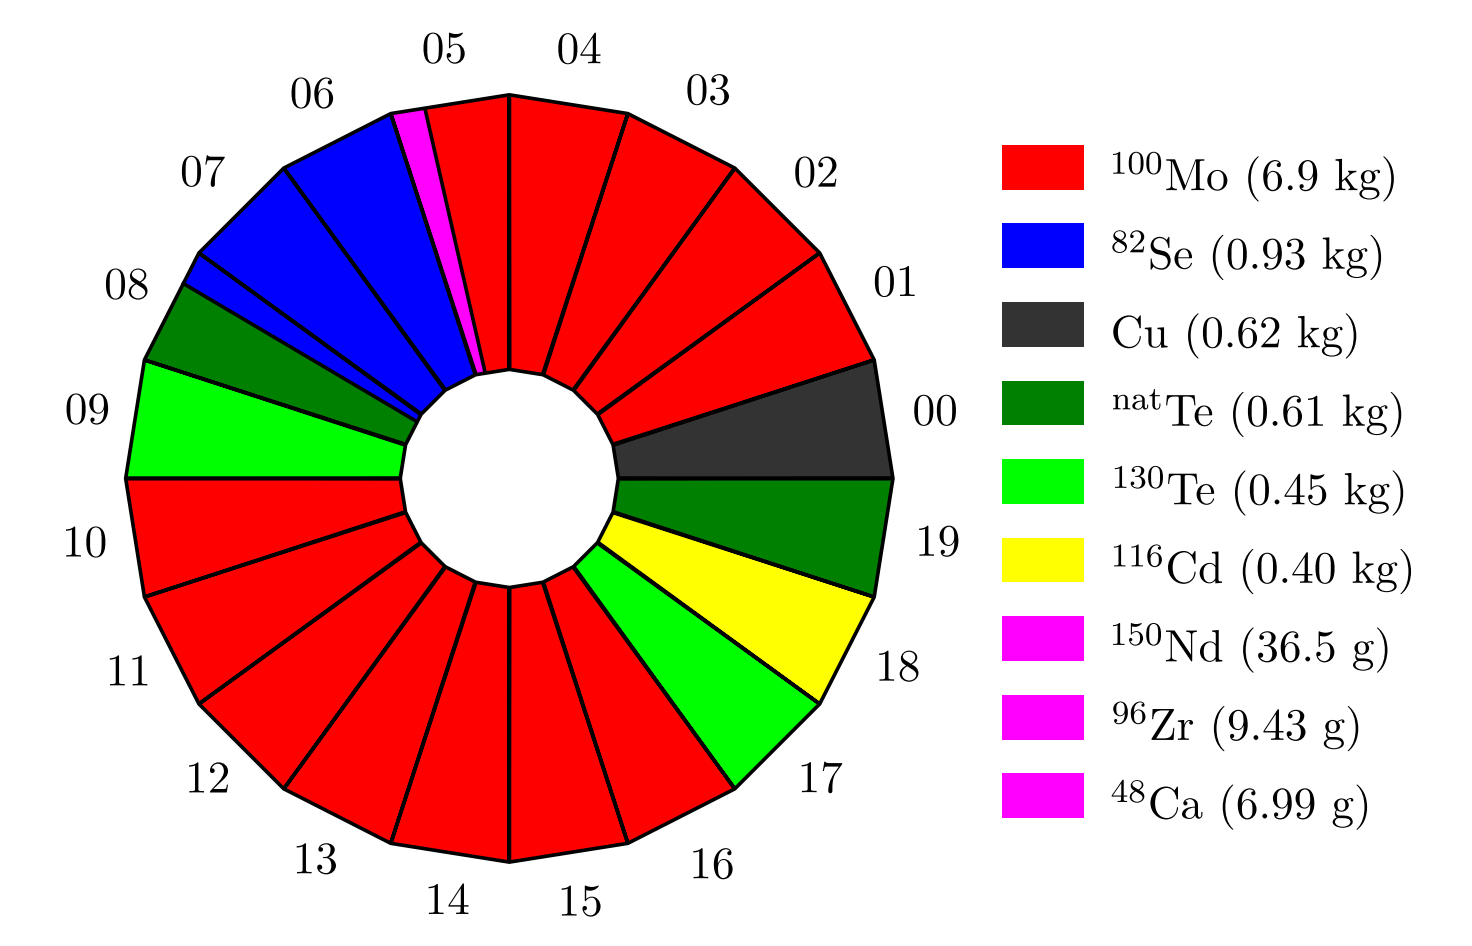
\includegraphics[scale=0.46]{pictures/Chap3/BBSourceDistribution.png}
\caption{Schematic view of the different $\beta\beta$ sources location inside the NEMO-3 detector.}
\label{NEMO3Sector}
\end{center}
\end{figure}


\FloatBarrier


\NI Each sector supports a source frame where 7 strips were placed. The mean length of the strips was 2.48~m. The width of the strips was 6.3~cm except for the 2 strips at the border (6.5~cm). The surface density of the source foils (equivalent to the thickness) had been determined from simulations. The detector efficiency for the 0$\nu\beta\beta$ process is not compromised
as long as the surface densities of the foils do not exceed 60 mg/cm$^\text{2}$ (limited by the energy resolution of the calorimeter). As consequence, the thickness of the metallic foils (cadmium, copper and a part of molybdenium) does not exceed 60~$\mu$m. The composite foils, which are a mixture of source powder and radiopure organic glue (selenium, tellurium, zirconium, neodynium and cadmium), does not exceed 300~$\mu$m. 


\bigskip


\NI All these $\beta\beta$ isotopes mainly provide from the Earth's crust (directly extracted or by-product of the extraction) and contain impurities ($^{\text{238}}$U and $^{\text{232}}$Th) which during their decay generate events similar to $\beta\beta$ events. To remove these impurities, the sample must be purify by physical or chemical technique. Some purification techniques are detailled in Appendix \ref{sec:PurificationMethods}.


\subsection{Tracking volume}


\NI The tracking volume is made of vertical layers of 6180 Geiger cells (for a total of 39820 wires). The diameter of the wires and the gas composition have been studied during a long time to optimize the resolution and the efficiency of the tracker. The number of wires shoud not be too large to improve the transparency and avoid multiple scattering effects. The composition of the gas must allow a good reconstruction efficiency, limit the energy loss and the aging of the cells. The gas is a mixture of 95 \% of helium, 4 \% of ethanol, 1 \% of argon and 0.1 \% of water. 


\bigskip


\NI In cross-sectional view, each cell has a octogonal geometry with a diameter of 3~cm. The central anode wire is surrounded by 8 ground wires (4 are in common with the adjecent cells to limit the number of wires). An extra ground wire have been added between the layers to avoid electrostatic cross talk. The wires are made of stainless steel, 2.7~m long and 50~$\mu$m in diameter, and are stung by two iron petals which form the top and the bottom of the detector. At each cell extremity, a  cathode ring (3~cm long and 2.3~cm in diameter) was placed, the anode wire runs through the center of this
ring while the ground wires are supported just outside. An elementary Geiger cell is shown in Figure~\ref{GeigerCellNEMO3}.


\begin{figure}[h!]
\begin{center}
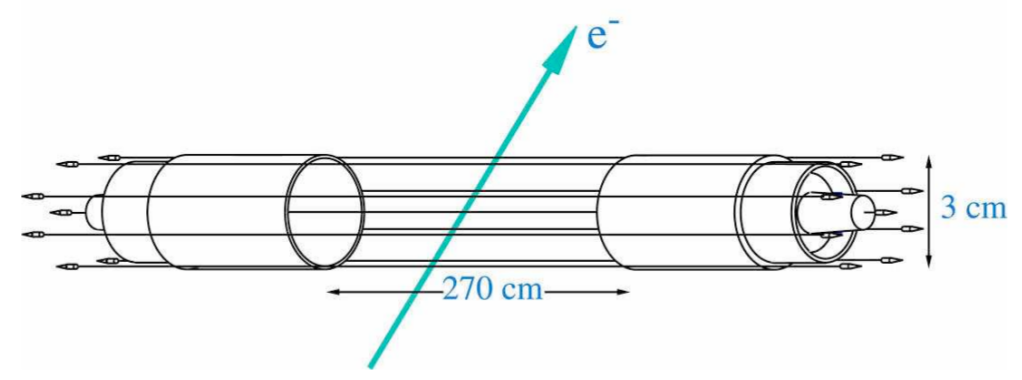
\includegraphics[scale=0.3]{pictures/Chap3/GeigerCellNEMO3.png}
\caption{Representation of an elementary Geiger cell in NEMO-3. The central anode wire is surrounded by 8 ground wires. The cathod rings are shown at each end of the cell.}
\label{GeigerCellNEMO3}
\end{center}
\end{figure}


\NI The operating voltage for the anode wires was $\sim$1800~V. In this condition, a crossing charged particle creates around 6 electrons per centimiter. Close to the anode, these electrons drift towards the anode wire at a speed of about 2.3 cm/$\mu$s. Far away from the anode wire, the mean drift velocity is around 1 cm/$\mu$s. As explained before, the transverse position of the particle in the cells is reconstructed with the measurements of the drift times. The avalanche near the anode wire develops into a Geiger plasma which propagates along the wire at a speed of 6 to 7 cm/$\mu$s. The propagation times are used to determine the longitudinal position of the particle.


\bigskip


\NI The wire chamber was configured as 18 layers of Geiger cells parallel to the source foil, 4-2-3 layers on each side, as shown in Figure~\ref{TrackerNEMOView}. This configuration have been optimised by Monte-Carlo simulations. First, 4 layers are close to the source to precisely reconstruct the vertex location. Then 2 middle layers allow a good measurement of the track curvature. Finally, 3 layers close to scintillators are used to determine the impact point on the block in order to correct the energy measurement and improve the energy resolution of the electrons (the light collection is not uniform according the impact point).   



\begin{figure}[h!]
\begin{center}
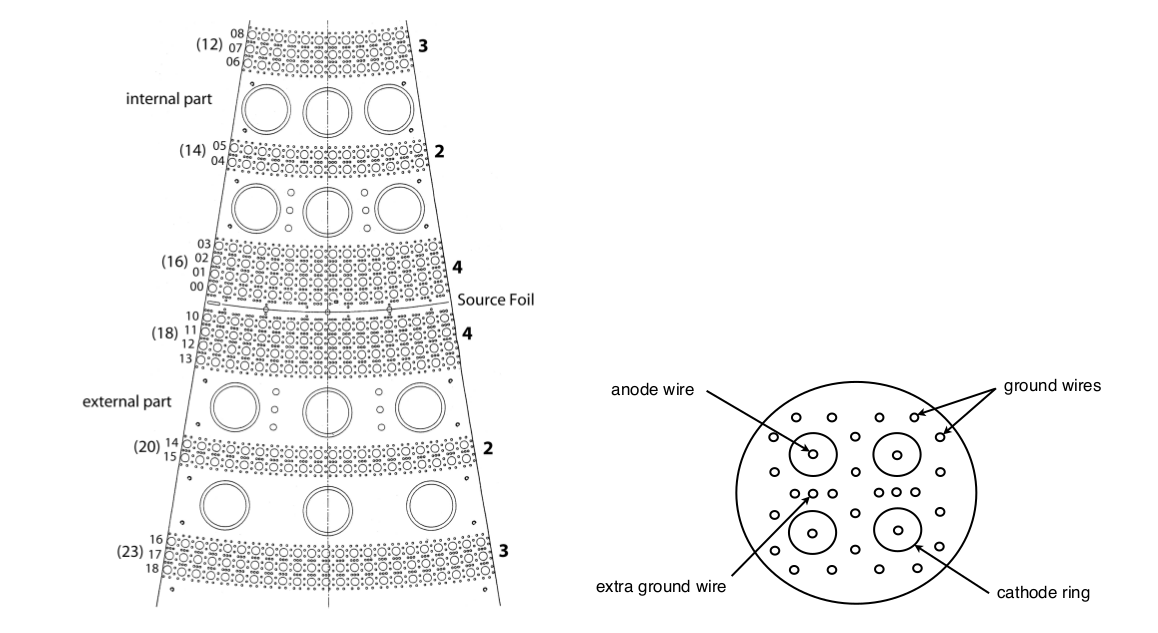
\includegraphics[scale=0.30]{pictures/Chap3/TrackerNEMOView.png}
\caption{Left : The 4-2-3 configuration of the Geiger cells in a NEMO-3 sector The 12 large rings represent the location of the light guides installed in the support structure to couple the scintillators to the PMTs. Right : Geiger
wiring of four elementary Geiger cells.}
\label{TrackerNEMOView}
\end{center}
\end{figure}


\FloatBarrier


\subsection{Calorimeter}


\NI The NEMO-3 calorimeter is made of 1940 optical modules to measure the particle energy, make time of flight measurements and give a fast trigger signal. Each of optical module is made with a plastic scintillator, light guide and PMT (3'' or 5''). As shown in Figure~\ref{NEMO3Inside},  the scintillators blocks covered the inner and outer cylindrical walls of the detector, and also had limited coverage on the top and bottom (call petals). The gains of the PMTs have been adjusted to cover energies up to 12 MeV. The plastic scintillators have been chosen to minimize backscattering and for their radiopurity.


\bigskip


\NI The scintillator was directly in contact with the gas of tracker. In order to prevent a rapid aging of the PMT due to the helium-alcohol gas, the blocks were supported by a rigid frame which allows the PMTs to be outside. To fit the cylindrical geometry of NEMO-3, 7 different types of scintillator have been specialy designed.


\bigskip


\NI The block are mainly made of a styrene polymere (C$_\text{6}$H$_\text{5}$CH=CH$_\text{2}$), with a mean Z of 3.7 per atom), 2~cm of this material is able to contain a up to 3~MeV electron. On the other hand, the mean Z is too low to optimise the photon interaction. The thickness of all the blocks have been set to 10~cm to obtain an efficiency for $\gamma$-ray detection of 50~\% at 500~keV. The chemical nature of the scintillator is a solid solution of a scintillating agent p-Terphenyl (PTP). Some 1.4-di-(5-phenyl-2-oxazoly) benzene (POPOP) is added in polystyrene to shift the wavelength for a better detection by the PMT ($\lambda \approx$ 420~nm). After many years of study, the final composition of the scintillation block have been chosen to be : 98.49~\% of polystyrene, 1.5~\% of PTP, and 0.01~\% of POPOP for the blocks of the walls and 98.75 \% of polystyrene, 1.2~\% of PTP, and 0.05~\% of POPOP for the petals blocks.


\bigskip


\NI The radiopurity of the scintillator blocks have measured to be 430 and 60 times better than the low radioactivity PMT (respectively in $^{\text{214}}$Bi and $^{\text{208}}$Tl). The blocks were finally wrapped with aluminized Mylar to not lose the scintillation light. A 60~mm thick light guide made of PMMA is used for the scintillator and PMT interface and to protect PMTs from helium. The light transmission through the guides is 98~\% in the wavelength range 380-420~nm.


\bigskip


\NI Based on analysis on NEMO-2 data, the dominant external background comes from the PMT. The development and the use of low radioactivity background is then crucial. For NEMO-3, the requirements for the PMT glass radioactivity was lower than 1.7~Bq/kg in $^{\text{40}}$K, lower than 0.83~Bq/kg in $^{\text{214}}$Bi and lower than 0.17~Bq/kg in $^{\text{208}}$Tl. The Hamamatsu company was chosen to produce the PMTs, with the radiopurity of their glass being 100 to 1000 times better than standard glass. Furthermore, the performances of their PMTs have been tested and meet the specifications : an energy resolution of 4~\% at 1~MeV, a time resolution of 250~ns at 1~MeV, a good linearity up to 4~MeV and a low dark current.  


\bigskip


\NI Two different kind of PMTs was used, the scintillator blocks of the internal walls and of the petals (except the petals close to the external wall) was coupled with R6091~3''~PMTs (1040 PMTs). These tubes are made of 12 dynodes and a flat photocathod. The blocks of the external wall and of the last petals were coupled to R6594~5''~PMTs (900 PMTs), having 10 dynodes and a hemispherical photocathode. A detailed schema of the location of the scintallator blocks in the NEMO-3 detector is presented in Figure~\ref{SectorDetailedPMTconfig}.


\bigskip


\begin{figure}[h!]
\begin{center}
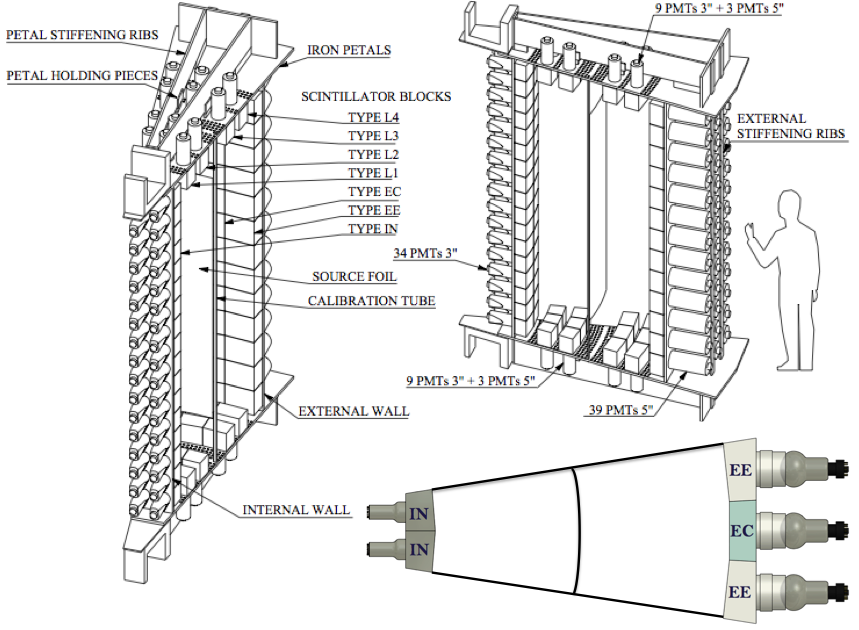
\includegraphics[scale=0.32]{pictures/Chap3/SectorDetailedPMTconfig.png}
\caption{One sector of NEMO 3 with details on the source foil, scintillator blocks and photomultipliers location.}
\label{SectorDetailedPMTconfig}
\end{center}
\end{figure}


\begin{figure}[h!]
\begin{center}
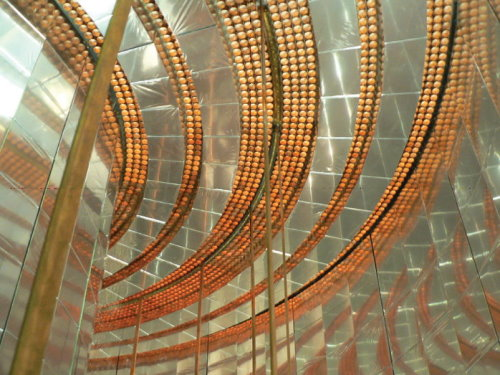
\includegraphics[scale=0.80]{pictures/Chap3/NEMO3Inside.jpg}
\caption{Inside view of the NEMO3 wire chamber during disassembly. The reflective surfaces are the calorimeter walls and the copper parts support the Geiger cell wires.}
\label{NEMO3Inside}
\end{center}
\end{figure}


\FloatBarrier


\subsection{Magnetic coil and shielding}


\NI In order to reach the desired sensitivity for the effective neutrino mass, no events of external background have to be seen in the energy range [2.8 - 3.2]~MeV during 5 years of data taking. The external background is induced by the interactions of neutrons and photons with the detector or with the rocks surrounded the laboratory. It will be more described in Section~\ref{sec:externalBkg}. 


\bigskip


\NI Simulations based on NEMO-3 geometry and studies from NEMO-2 shown that the photon interaction with the source foil mainly generate a pair creation (e$^+$e$^-$) [ref : C. Marquet et al., NEMO collaboration, Nucl. Instr. and Meth. A457(2001) 487]. The installation of a solenoid capable of producing a 25~G magnetic field surrounded by external shields highly reduce the external background. The magnetic coil allows positron/electron discrimation during the shields stop the majority of photons and neutrons.  


\subsubsection{The magnetic coil}


\NI The magnetic field have been optimized to maintain a good electron detection efficiency and distinguish the charge of the particles. In case where the magnetic field is too intense, the electrons are too curved and can not reach the calorimeter. On the other hand, the field must be sufficient to curve the trajectory for a good charge discrimation. An chosen value of 25~G provides a rejection of 95~\% of the (e$^+$e$^-$) pair event.


\bigskip


\NI The cylindrical coil surronds entirely the detector is made of 10 sections with 203 copper rings connecting every other sector to form one loop of the helix as shown in Section~\ref{NEMO3Detector}. The coil is 5320 mm in diameter, 2713 mm in height and has a mass of 5 tons ($\sim$ 3.1 tons of high radiopurity copper). To generate 25~G the required current is 29~A, and by taking account the resistivity of the copper rings (1.6 $\times$ 10$^{\text{-8}}$~$\Omega$), the total resistance of the coil is 0.6~$\Omega$. Fans have been placed in each section of the iron shield (Flow rate 1~m$^\text{3}$/s) are sufficient to cool the coil and the PMTs.



\subsubsection{The shieldings}


\NI To restrain the troublesome flux of photons and neutrons two shields have been installed. The first one is made of 20~cm (18~cm at few places to fit with the mechanical support) of radiopure iron spit into ten sections (165 tons) with two end-caps (6 tons each). This first shield reduces the $\gamma$-ray and thermal neutron fluxes. The second one have been optimized to suppress the contribution of slow and fast neutrons (up to few MeV). It is made itself of 3 parts :  20~cm of paraffin located below the central tower of the detector (not shown in Figure~\ref{NEMO3Detector}), 28~cm of wood placed below and above the detector, and 35~cm of borated water contained in tank covered the walls of the detector.  



\subsection{Calibration system}

\NI To distinguish true 0$\nu\beta\beta$ events from various background processes (2$\nu\beta\beta$ decay is only experimentaly differentiable from 0$\nu\beta\beta$ by energy), a good calorimeter energy resolution is important. Thus a robust calibration procedure is needed to ensure and monitor the response of the calorimeter and detect any changes over the lifetime of the experiment. The NEMO-3 solution is the use of radioactive sources introduced inside the detector during runs dedicated to calibration. The absolute energy scale is determined during these runs (approximately one day every month), but the rest of the time, a laser survey system control the stability of the optical modules. 


\bigskip


\NI To introduce different calibration sources into the detector each sectors was equiped with a vertical tube made of flattened copper located along the edge of the source foils. The sources were placed along a narrow delrin rod (3 per rod at z~=~-90, 0 and +90~cm), and introduced by the top of the detector (after the removal of some shields). The position of the sources have been chosen to obain an uniform illumination of the scintillator blocks. This system allow to place the calibration sources close the $\beta\beta$ foils, thus the electron trajectories are very similar to the expected tracks in $\beta\beta$ events.


\bigskip


\NI 






\subsection{Results and measurements}

\section{SuperNEMO}\label{sec:SuperNEMO}
\subsection{$^{\text{82}}$Se source foils}
\subsection{Tracking volume}
\subsection{Calorimeter}
\subsection{Radiopurity constains}
\subsection{Shielding and gas system}
\subsection{Prospectives}


\end{document}
